\documentclass[polish,polish,a4paper]{article}
\usepackage[polish]{babel}
\usepackage[T1]{fontenc}
\usepackage[utf8]{inputenc}
\usepackage{pslatex}
\usepackage{pgfplots}
\usepackage{circuitikz} 
\usepackage{setspace}
\usepackage{caption}
\usepackage{amssymb}
\usepackage{amsmath}
%\usetikzlibrary{circuits.ee.IEC}
\usepackage{anysize}
\usepackage{graphicx}
\usepackage{hyperref}
\usepackage{float}
\usepackage{color}
\usepackage{multirow}
\hypersetup{
	colorlinks=true,
	linkcolor=blue,
	filecolor=magenta,      
	urlcolor=cyan,
}

\marginsize{2.5cm}{2.5cm}{2cm}{2cm}

\newcommand{\PRzFieldDsc}[1]{\sffamily\bfseries\scriptsize #1}
\newcommand{\PRzFieldCnt}[1]{\textit{#1}}
\newcommand{\PRzHeading}[8]{
	%% #1 - nazwa laboratorium
	%% #2 - kierunek 
	%% #3 - specjalność 
	%% #4 - rok studiów 
	%% #5 - symbol grupy lab.
	%% #6 - temat 
	%% #7 - numer lab.
	%% #8 - skład grupy ćwiczeniowej
	
	\begin{center}
		\begin{tabular}{ p{0.32\textwidth} p{0.15\textwidth} p{0.15\textwidth} p{0.12\textwidth} p{0.12\textwidth} }
			
			&   &   &   &   \\
			\hline
			\multicolumn{5}{|c|}{}\\[-1ex]
			\multicolumn{5}{|c|}{{\LARGE #1}}\\
			\multicolumn{5}{|c|}{}\\[-1ex]
			
			\hline
			\multicolumn{1}{|l|}{\PRzFieldDsc{Kierunek}}	& \multicolumn{1}{|l|}{\PRzFieldDsc{Specjalność}}	& \multicolumn{1}{|l|}{\PRzFieldDsc{Rok studiów}}	& \multicolumn{2}{|l|}{\PRzFieldDsc{Symbol grupy lab.}} \\
			\multicolumn{1}{|c|}{\PRzFieldCnt{#2}}		& \multicolumn{1}{|c|}{\PRzFieldCnt{#3}}		& \multicolumn{1}{|c|}{\PRzFieldCnt{#4}}		& \multicolumn{2}{|c|}{\PRzFieldCnt{#5}} \\
			
			\hline
			\multicolumn{4}{|l|}{\PRzFieldDsc{Temat Laboratorium}}		& \multicolumn{1}{|l|}{\PRzFieldDsc{Numer lab.}} \\
			\multicolumn{4}{|c|}{\PRzFieldCnt{#6}}				& \multicolumn{1}{|c|}{\PRzFieldCnt{#7}} \\
			
			\hline
			\multicolumn{5}{|l|}{\PRzFieldDsc{Skład grupy ćwiczeniowej oraz numery indeksów}}\\
			\multicolumn{5}{|c|}{\PRzFieldCnt{#8}}\\
			
			\hline
			\multicolumn{3}{|l|}{\PRzFieldDsc{Uwagi}}	& \multicolumn{2}{|l|}{\PRzFieldDsc{Ocena}} \\
			\multicolumn{3}{|c|}{\PRzFieldCnt{\ }}		& \multicolumn{2}{|c|}{\PRzFieldCnt{\ }} \\
			
			\hline
		\end{tabular}
	\end{center}
}



\begin{document}

\begin{spacing}{1.3}


	\PRzHeading{Laboratorium Podstaw Elektroniki}{Informatyka}{--}{I}{I3}{Wzmacniacze operacyjne}{8}{Piotr Więtczak(132339), Robert Ciemny(136693), Kamil Basiukajc(136681)}

\

\section{PLAYGROUND}

\begin{gather*}
%
1. \quad U_{out} = k_{u} \cdot U_{in} = k_{u}(U_{A} - U_{B})\\
%
2. \quad \dfrac{U_{out}(s)}{U_{in}(s)} = 1 + \dfrac{Z_{f}}{Z_{in}}\\
%
3. \quad \dfrac{U_{out}(s)}{U_{in}(s)} = - \dfrac{Z_{f}}{Z_{in}}\\
%
4. \quad Z_{f} = \dfrac{1}{sC}\\
%
5. \quad \dfrac{U_{out}(s)}{U_{in}(s)} = - \dfrac{\dfrac{1}{sC}}{R} = - \dfrac{1}{RC} \cdot \dfrac{1}{s}\\
%
6. \quad u_{out}(t) = - \dfrac{1}{RC} \int u_{in}(t)dt = - \dfrac{1}{T_{i}} \int u_{in}(t)dt\\
%
7. \quad Z_{in} = \dfrac{1}{sC}\\
%
8. \quad \dfrac{U_{out}(s)}{U_{in}(s)} = - \dfrac{R}{\dfrac{1}{sC}} = - RC \cdot s\\
%
9. \quad u_{out}(t) = -RC\dfrac{du_{in}(t)}{dt} = -T_{d}\dfrac{du_{in}(t)}{dt}
\end{gather*}

\section{Wstęp do laboratoriów}

Po zapoznaniu się z treścią zaprezentowanego pdfa, złożono układ do badań zgodnie z instrukcjami i po sprawdzeniu połączonego układu przez prowadzącego przystąpiono do dalszych zadań. Prowadzący wybrał dla naszej grupy laboratoryjnej częstotliwość $1kHz$.

\section{Konfiguracja nieodwracająca} %1.3.1

\subsection{Cel zadania}

Badanie wzmacniacza operacyjnego w konfiguracji nieodwracającej.

\subsection{Przebieg zadania}

\begin{figure}[H]
	\begin{equation*}
	\begin{circuitikz}
	\draw
	(0,0) node[op amp] (pap) {}
	(pap.out) to [short,-o] (2,0)
	(-2,-0.5) to [short, o-] (pap.+)
	(-3,0.5) to [european resistor, l=$Z_{in}$] 
	(pap.-) to (-1.2,2)
	to [european resistor, l = $Z_{f}$] (1.2,2)
	to (pap.out)
	(-3,0.4) to (-3,0.6);
	\end{circuitikz}
	\end{equation*}
	\captionof{figure}{Konfiguracja nieodwracająca}
\end{figure}

Przygotowano układ zgodnie z instrukcjami i odczytano wartości elementów rezystancyjnych $R_{1} = 1k\Omega$ ( wartość z pomiarów $987.573\Omega$ ), $R_{2} = 1k\Omega$ ( wartość z pomiarów $992.386\Omega$)  odpowiedzialnych za wyznaczenie stopnia wzmocnienia w tej konfiguracji.

Za pomocą oscyloskopu odczytano amplitudy przebiegów wejściowego $500mV$ i wyjściowego $1V$, a następnie zapisano ich oscylogram

\begin{figure}[H]
	\centering
	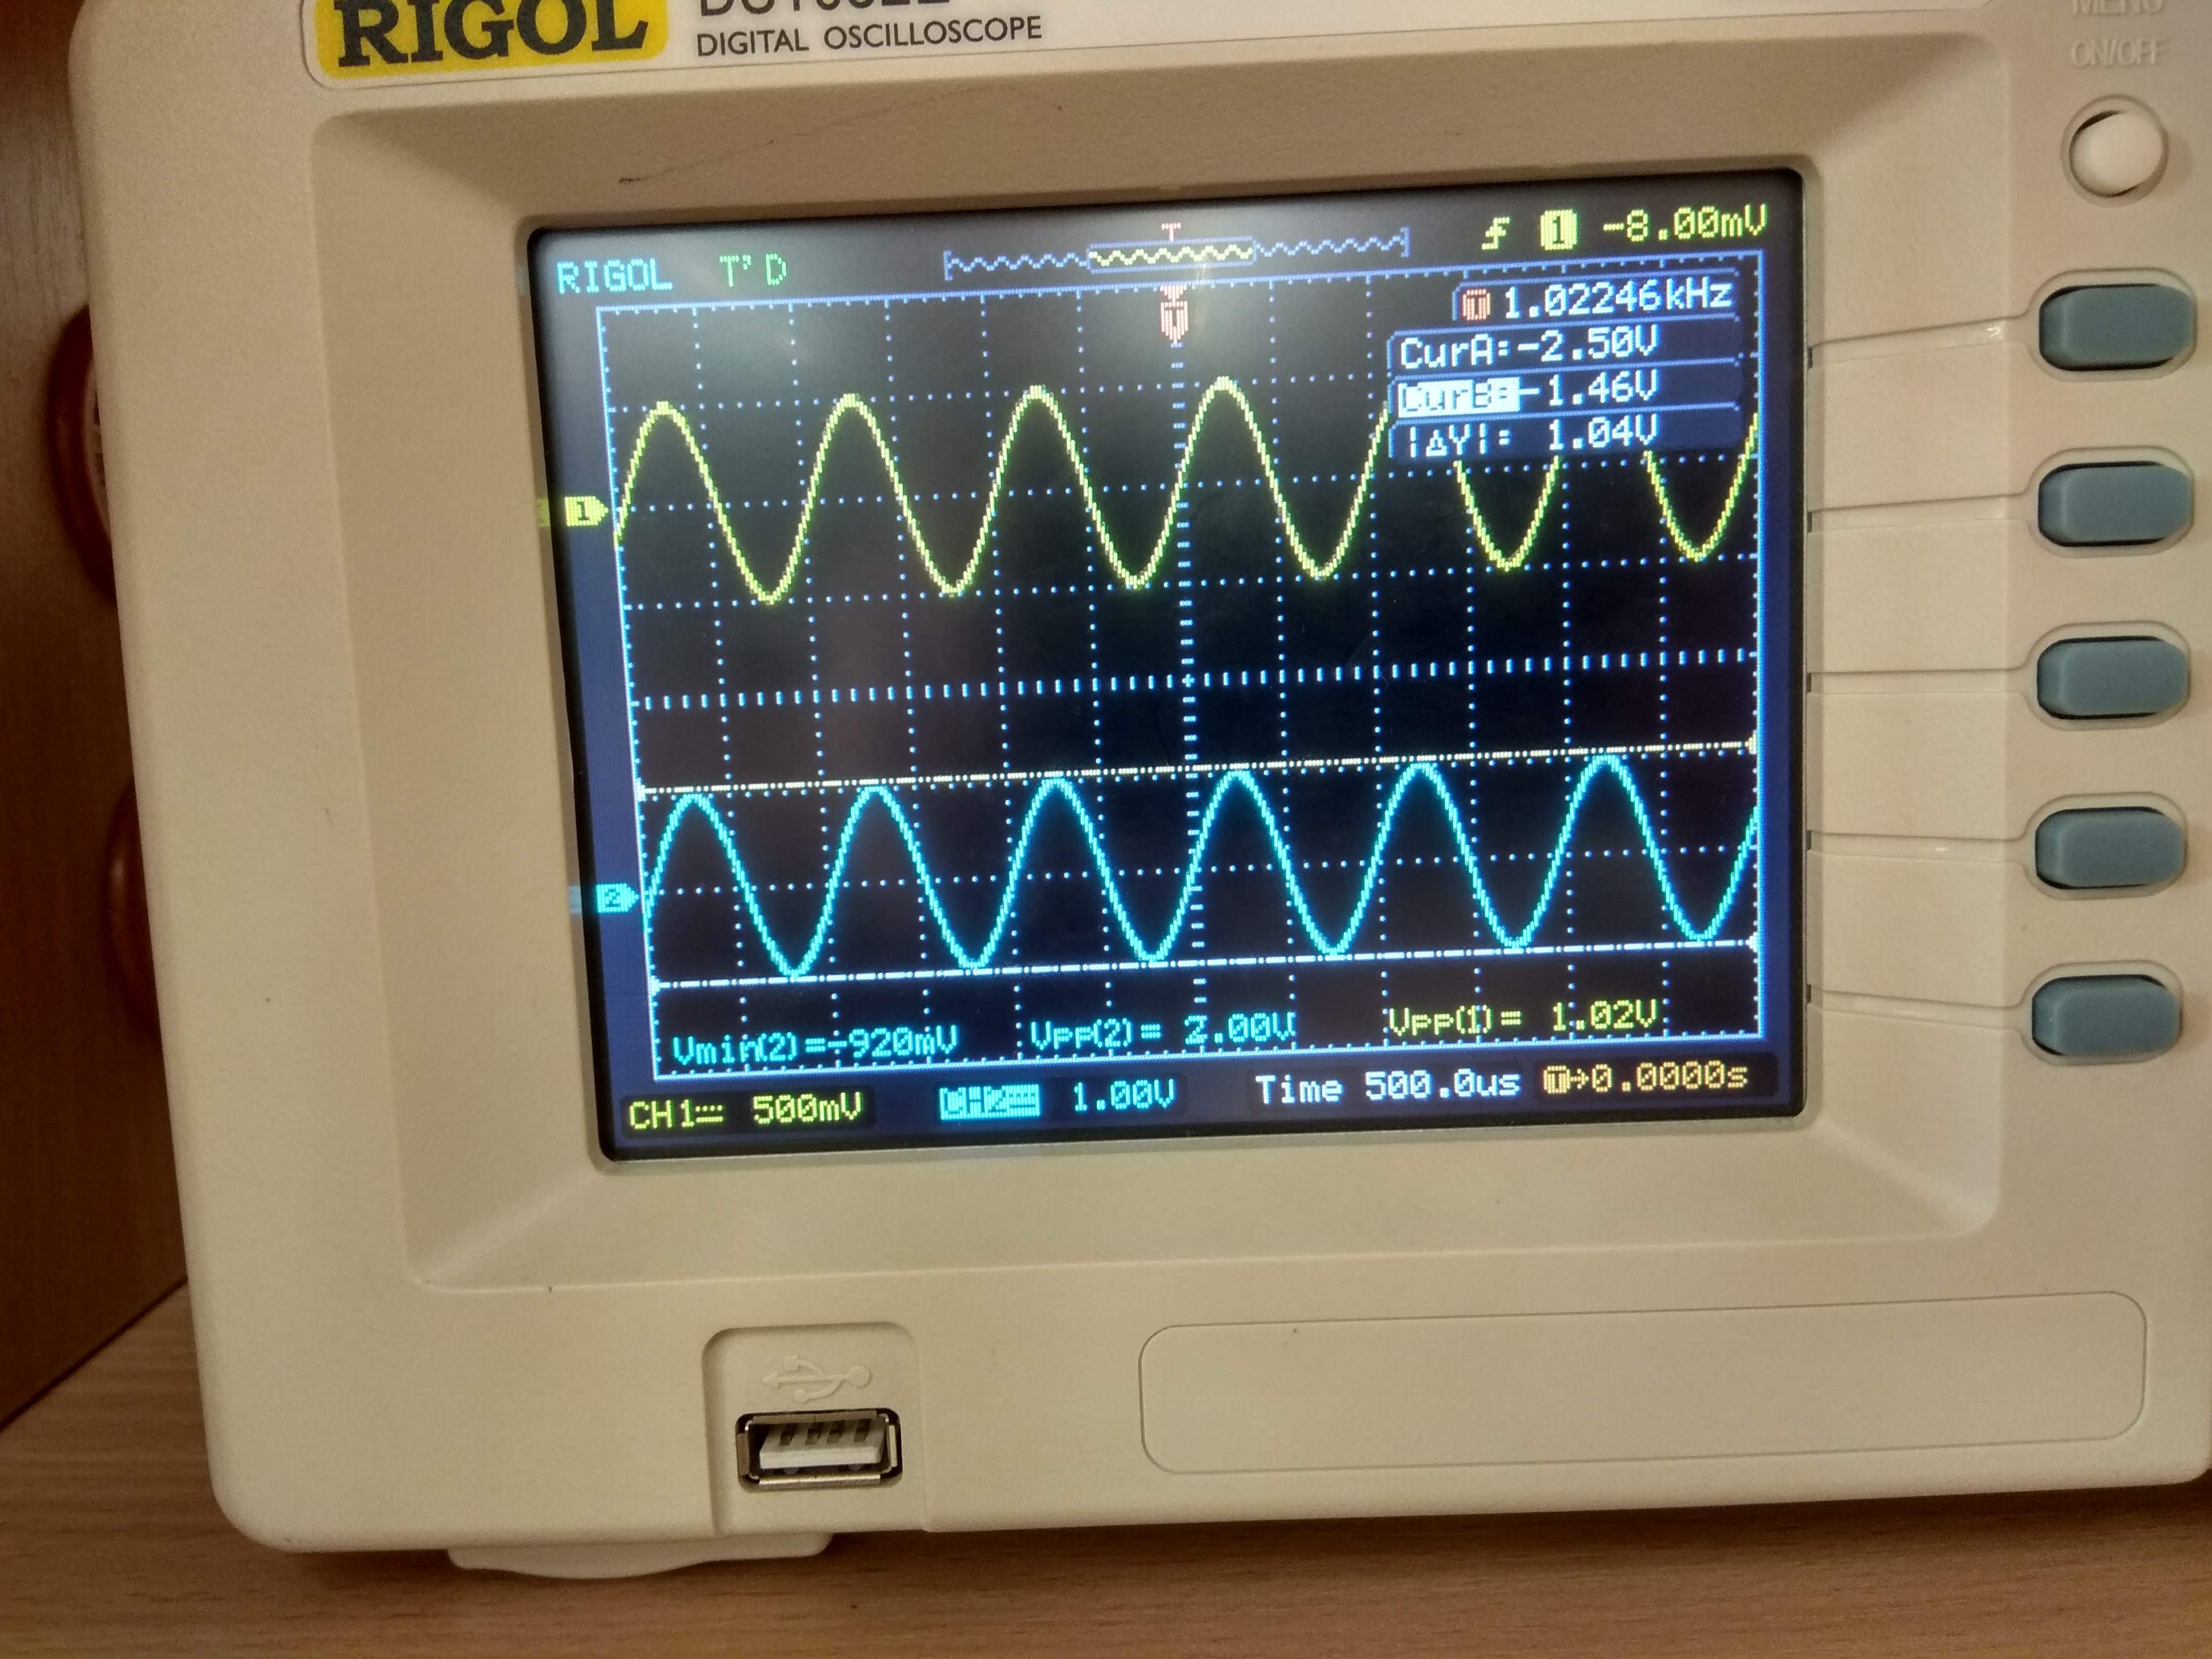
\includegraphics[scale=0.1]{131.jpg}
	\captionof{figure}{Zapisany oscylogram wybranej pary przebiegów.}
\end{figure}

Wzmocnienie oszacowano na $2$ w skali linowej i $10 \log_{10} 2 \approx 3.0103 dB$

Za pomocą zależności $\dfrac{U_{out}(s)}{U_{in}(s)} = 1 + \dfrac{Z_{f}}{Z_{in}} = 2 $  porównano wartość wzmocnienia z zależnością.

Na podstawie ogólnego równania opisującego wzmocnienie stopnia w konfiguracji nieodwracającej, $\dfrac{U_{out}(s)}{U_{in}(s)} = 1 + \dfrac{Z_{f}}{Z_{in}}$, określono że wzmocnienie dla układu wtórnika napięciowego jest równe $1$. 

Wtórnik napięcia prawie wcale nie pobiera prądu ze źródła sygnału, a umożliwia pobranie całkiem sporego prądu ze swojego wyjścia, przez co układy te są stosowane w celu odseparowania źródła sygnału od odbiornika.


\subsection{Wnioski}

Po przeanalizowaniu oszacowanych wartości z teoretycznymi stwierdzono, ze doświadczenie przeprowadzono poprawnie.

\section{Konfiguracja odwracająca} %1.4.1

\subsection{Cel zadania}

Badanie wzmacniacza operacyjnego w konfiguracji odwracającej

\subsection{Przebieg zadania}


\begin{figure}[H]
	\begin{equation*}
	\begin{circuitikz}
	\draw
	(0,0) node[op amp] (pap) {}
	(pap.out) to [short,-o] (2,0)
	(-2,-0.5) to (pap.+)
	(-3,0.5) to [short, o-, european resistor, l=$Z_{in}$] 
	(pap.-) to (-1.2,2)
	to [european resistor, l = $Z_{f}$] (1.2,2)
	to (pap.out)
	(-2,-0.4) to (-2,-0.6);
	\end{circuitikz}
	\end{equation*}
	\captionof{figure}{Konfiguracja odwracająca}
\end{figure}

Przygotowano układ zgodnie z instrukcjami i odczytano wartości elementów rezystancyjnych i pojemnościowych możliwych do załączenia w roli impedancji $Z_{f}$ oraz $Z_{in}$ w tej konfiguracji.

\begin{spacing}{1.5}
	\begin{equation*}
	\begin{array}{|l|c|l|}
	\hline
	\multicolumn{1}{|c|}{$nazwa$}&\multicolumn{1}{|c|}{Z_{in}/}&\multicolumn{1}{|c|}{$wartości$}\\
	\multicolumn{1}{|c|}{$elementu$}&\multicolumn{1}{|c|}{Z_{f}}&\multicolumn{1}{|c|}{$odczytów$}\\
	\hline
	R3&\multirow{4}{*}{$Z_{in}$}&1k\Omega\\
	C1&&100nF\\
	R4&&2k\Omega\\
	R5&&1k\Omega\\\hline
	C2&\multirow{4}{*}{$Z_{f}$}&10nf\\
	R6&&5k\Omega\\
	R7&&1k\Omega\\
	R8&&2k\Omega\\\hline
	\end{array}
	\end{equation*}
		\captionof{table}{Zestawienie dokonanych pomiarów i odczytów.}
\end{spacing}

Przy pomocy oscyloskopu odczytano wartości $u_{we}$ i $w_{wy}$, następnie obliczono $k_{u}$ przy pomocy wzoru $\dfrac{U_{out}(s)}{U_{in}(s)} = - \dfrac{Z_{f}}{Z_{in}}$, dla rożnych ustawień wzmacniacza.

\begin{spacing}{1.8}
	\begin{equation*}
	\begin{array}{|l|l|l|l||l|l|l|l|l|}
	\hline
	\multicolumn{1}{|c|}{Z_{in}}&\multicolumn{1}{c|}{$nr przełącznika$}&\multicolumn{1}{c|}{Z_{f}}&\multicolumn{1}{c||}{$nr przełącznika$}&
	\multicolumn{1}{|c|}{k_{u} $ teoretyczne$}&\multicolumn{1}{c|}{u_{we}}&\multicolumn{1}{c|}{u_{wy}}&\multicolumn{1}{c|}{k_{u}$ $ [V/V]}&\multicolumn{1}{c|}{k_{u} $ $ [dB]}\\
	\hline
	1k\Omega&1&2k\Omega&1&-2&1.06V&-2.12V&-2&-3.01\\
	1k\Omega&1&1k\Omega&2&-1&1.06V&-1.06V&-1&0\\
	1k\Omega&1&5k\Omega&3&-5&1.06V&-5.44V&-5.13&-7.10\\
	2k\Omega&2&1k\Omega&2&-0.5&1.06V&-0.54V&-0.5&3.01\\
	\hline
	\end{array}
	\end{equation*}
	\captionof{table}{Zestawienie danych pomiarowych i obliczeniowych stopnia wzmacniającego.}
\end{spacing}



Zapisano oscylogram wybranej pary przebiegów, dla $Z_{in}$ numer przełącznika: $1$ i $Z_{f}$ numer przełącznika: $2$.

\begin{figure}[H]
	\centering
	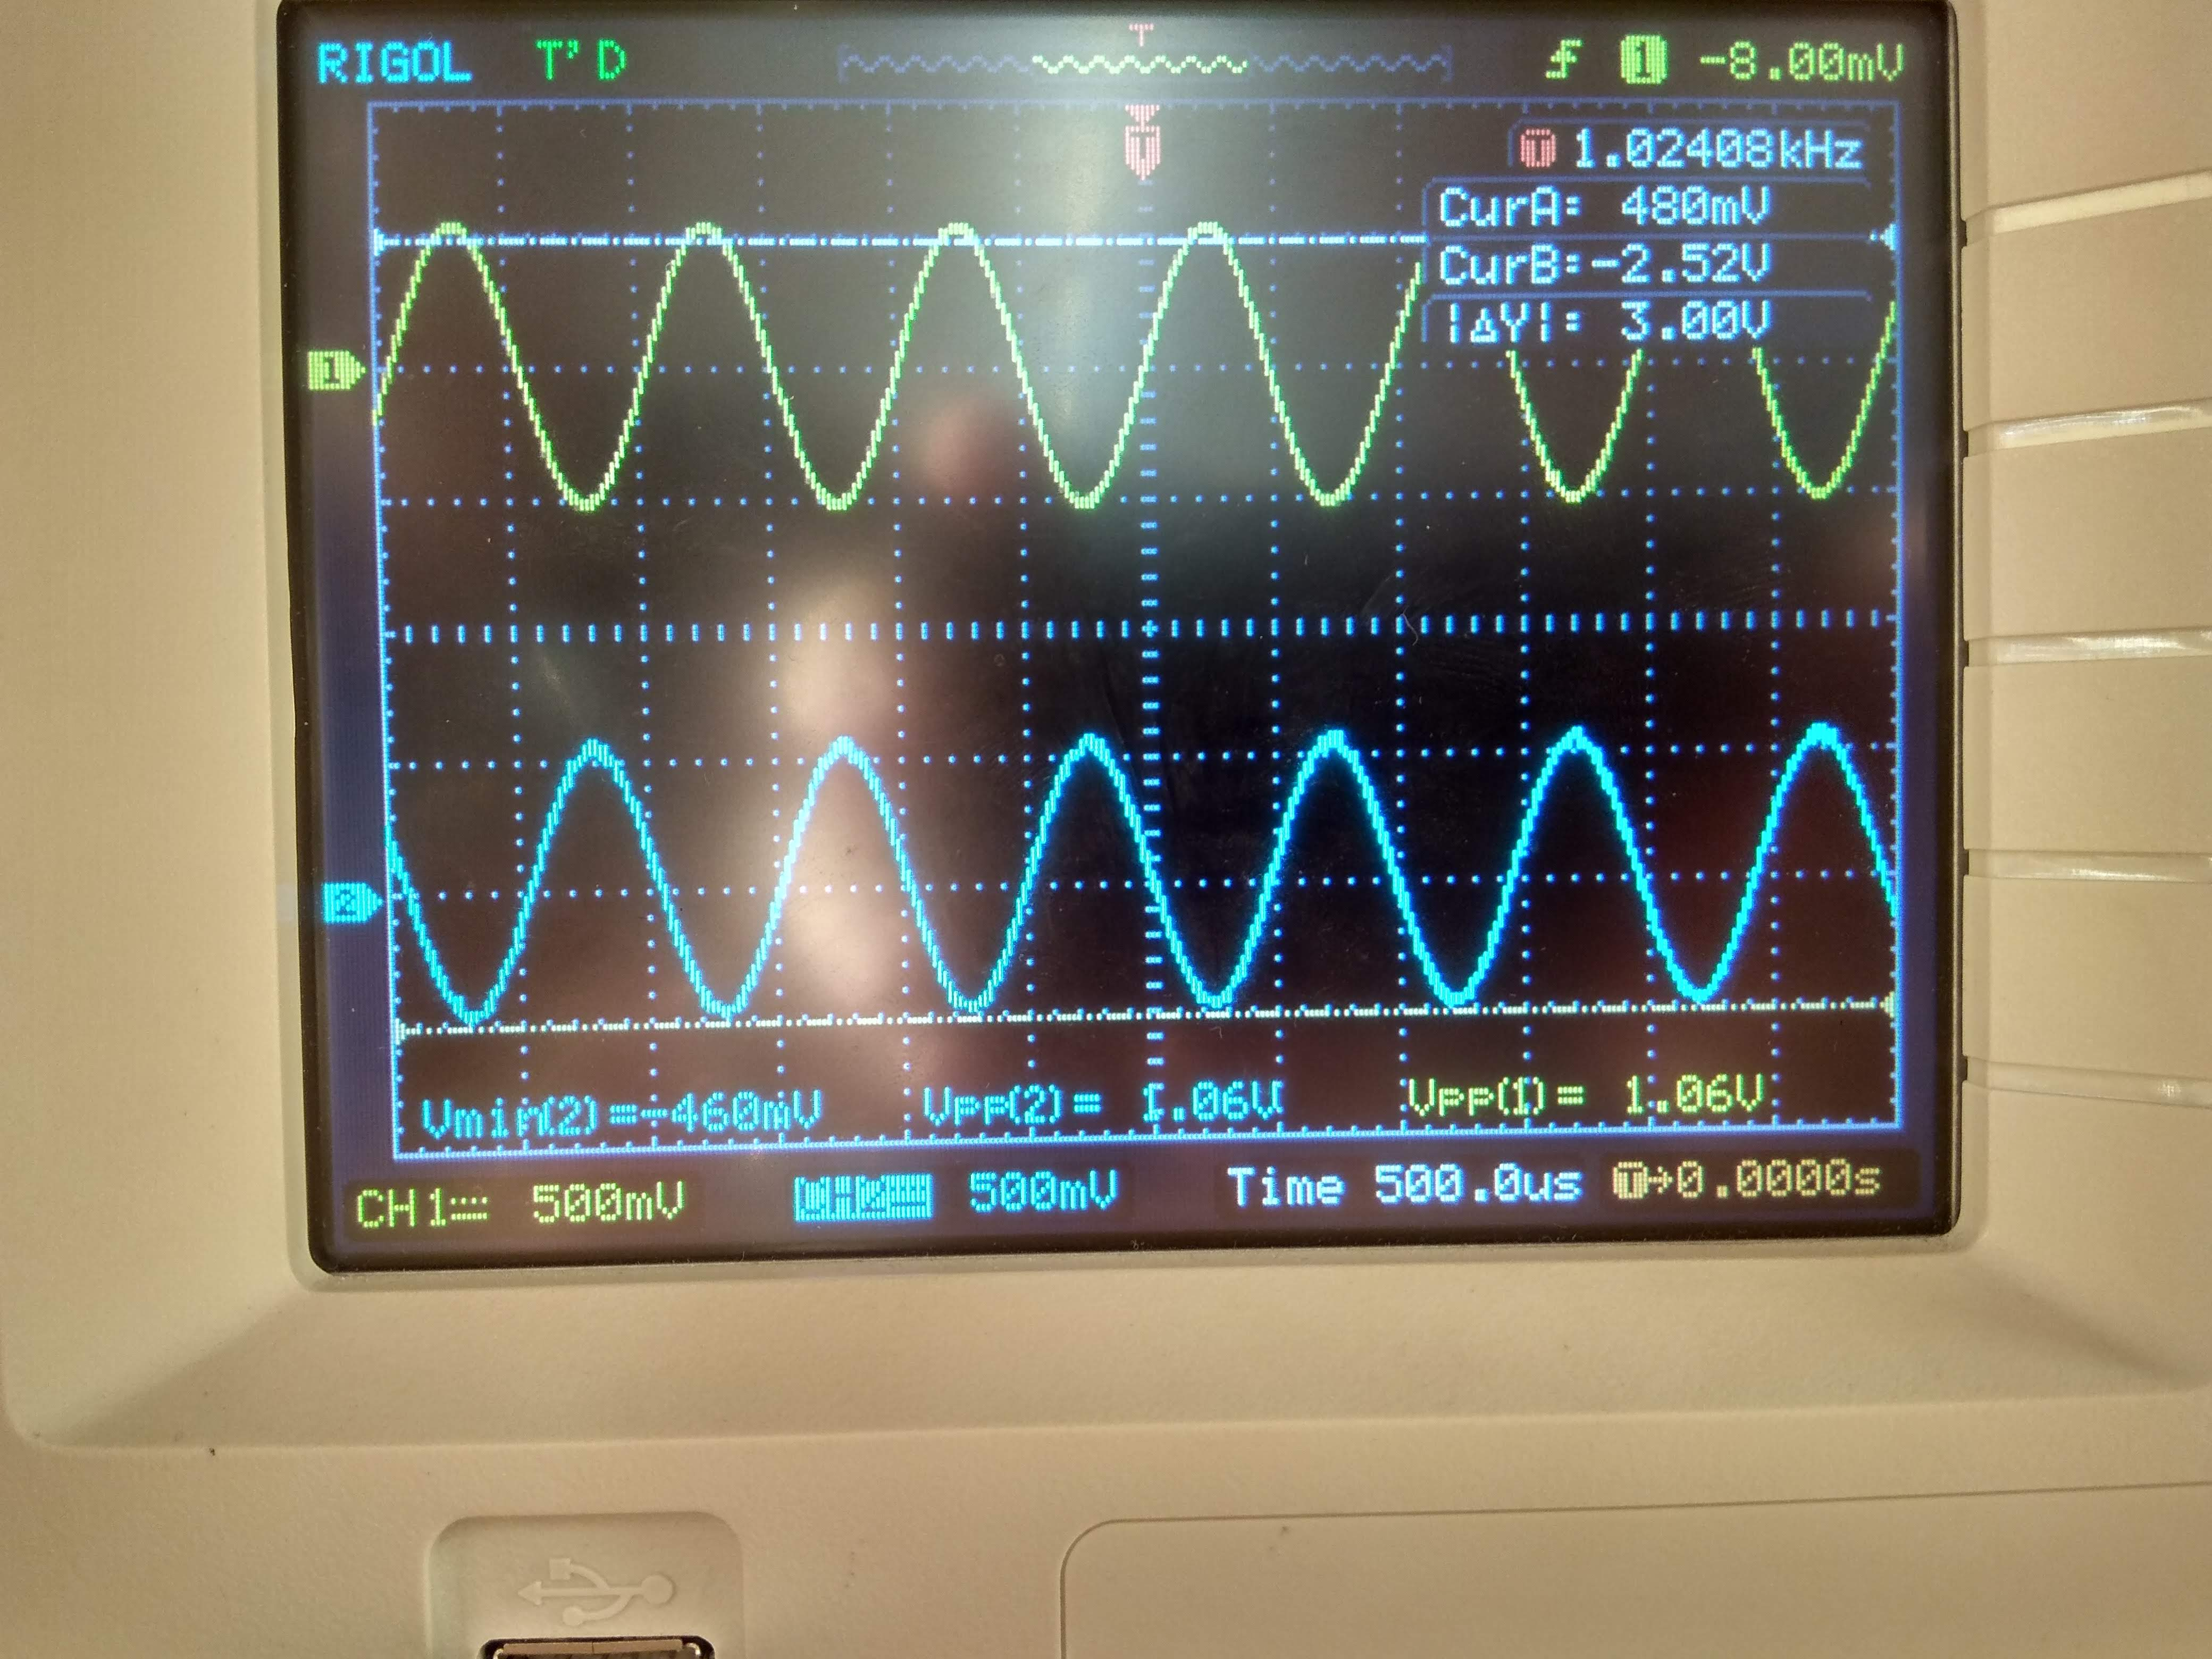
\includegraphics[scale=0.1]{141.jpg}
	\captionof{figure}{Zapisany oscylogram dla wybranej pary przebiegów.}
\end{figure}

Różnice między teoretyczną a uzyskaną wartością pomiarów wzmocnienia $k_{u}$, wynikają z niedokładnością sprzętu pomiarowego i elementów układu.

Przesunięcie fazowe między przebiegami wynosi $\Pi$ i jest spowodowane różnicą napięć

\subsection{Wnioski}

Po przeanalizowaniu oszacowanych wartości z teoretycznymi stwierdzono, ze doświadczenie przeprowadzono poprawnie.

\section{Blok integratora} %1.5.1

\subsection{Cel zadania}

Badanie układu całkującego.

\subsection{Przebieg zadania}

Przygotowano układ zgodnie z instrukcjami i za pomocą oscyloskopu odczytano współczynniki nachylenia przebiegu trójkątnego.

Korzystając z zależności $\quad u_{out}(t) = - \dfrac{1}{RC} \int u_{in}(t)dt = - \dfrac{1}{T_{i}} \int u_{in}(t)dt$ wyprowadzono wzór $\dfrac{1}{T_{i}} = \dfrac{1}{RC}$ do obliczenia teoretycznego $ \dfrac{1}{T_{i}}$
\begin{spacing}{2}
\begin{equation*}
\begin{array}{|r|r|r|r||r|r|}
\hline
\multicolumn{1}{|c|}{R}&\multicolumn{1}{c|}{$nr przełącznika$}&\multicolumn{1}{c|}{C}&\multicolumn{1}{c||}{$nr przełącznika$}&
\multicolumn{1}{c|}{\dfrac{1}{T_{i}}$ teoretyczne$}&\multicolumn{1}{c|}{\dfrac{1}{T_{i}}$ obliczone$}\\
\hline

1k\Omega&1&10nF&4&-&-\\
2k\Omega&2&10nF&4&-&-\\
\hline

\end{array}
\end{equation*}
\captionof{table}{Zestawienie danych pomiarowych i obliczeniowych stopnia wzmacniającego.}
\end{spacing}

Zapisano oscylogram wybranej pary przebiegów: wejściowego i wyjściowego, dla $R = 2k\Omega$, $C = 10nF$.

\begin{figure}[H]
	\centering
	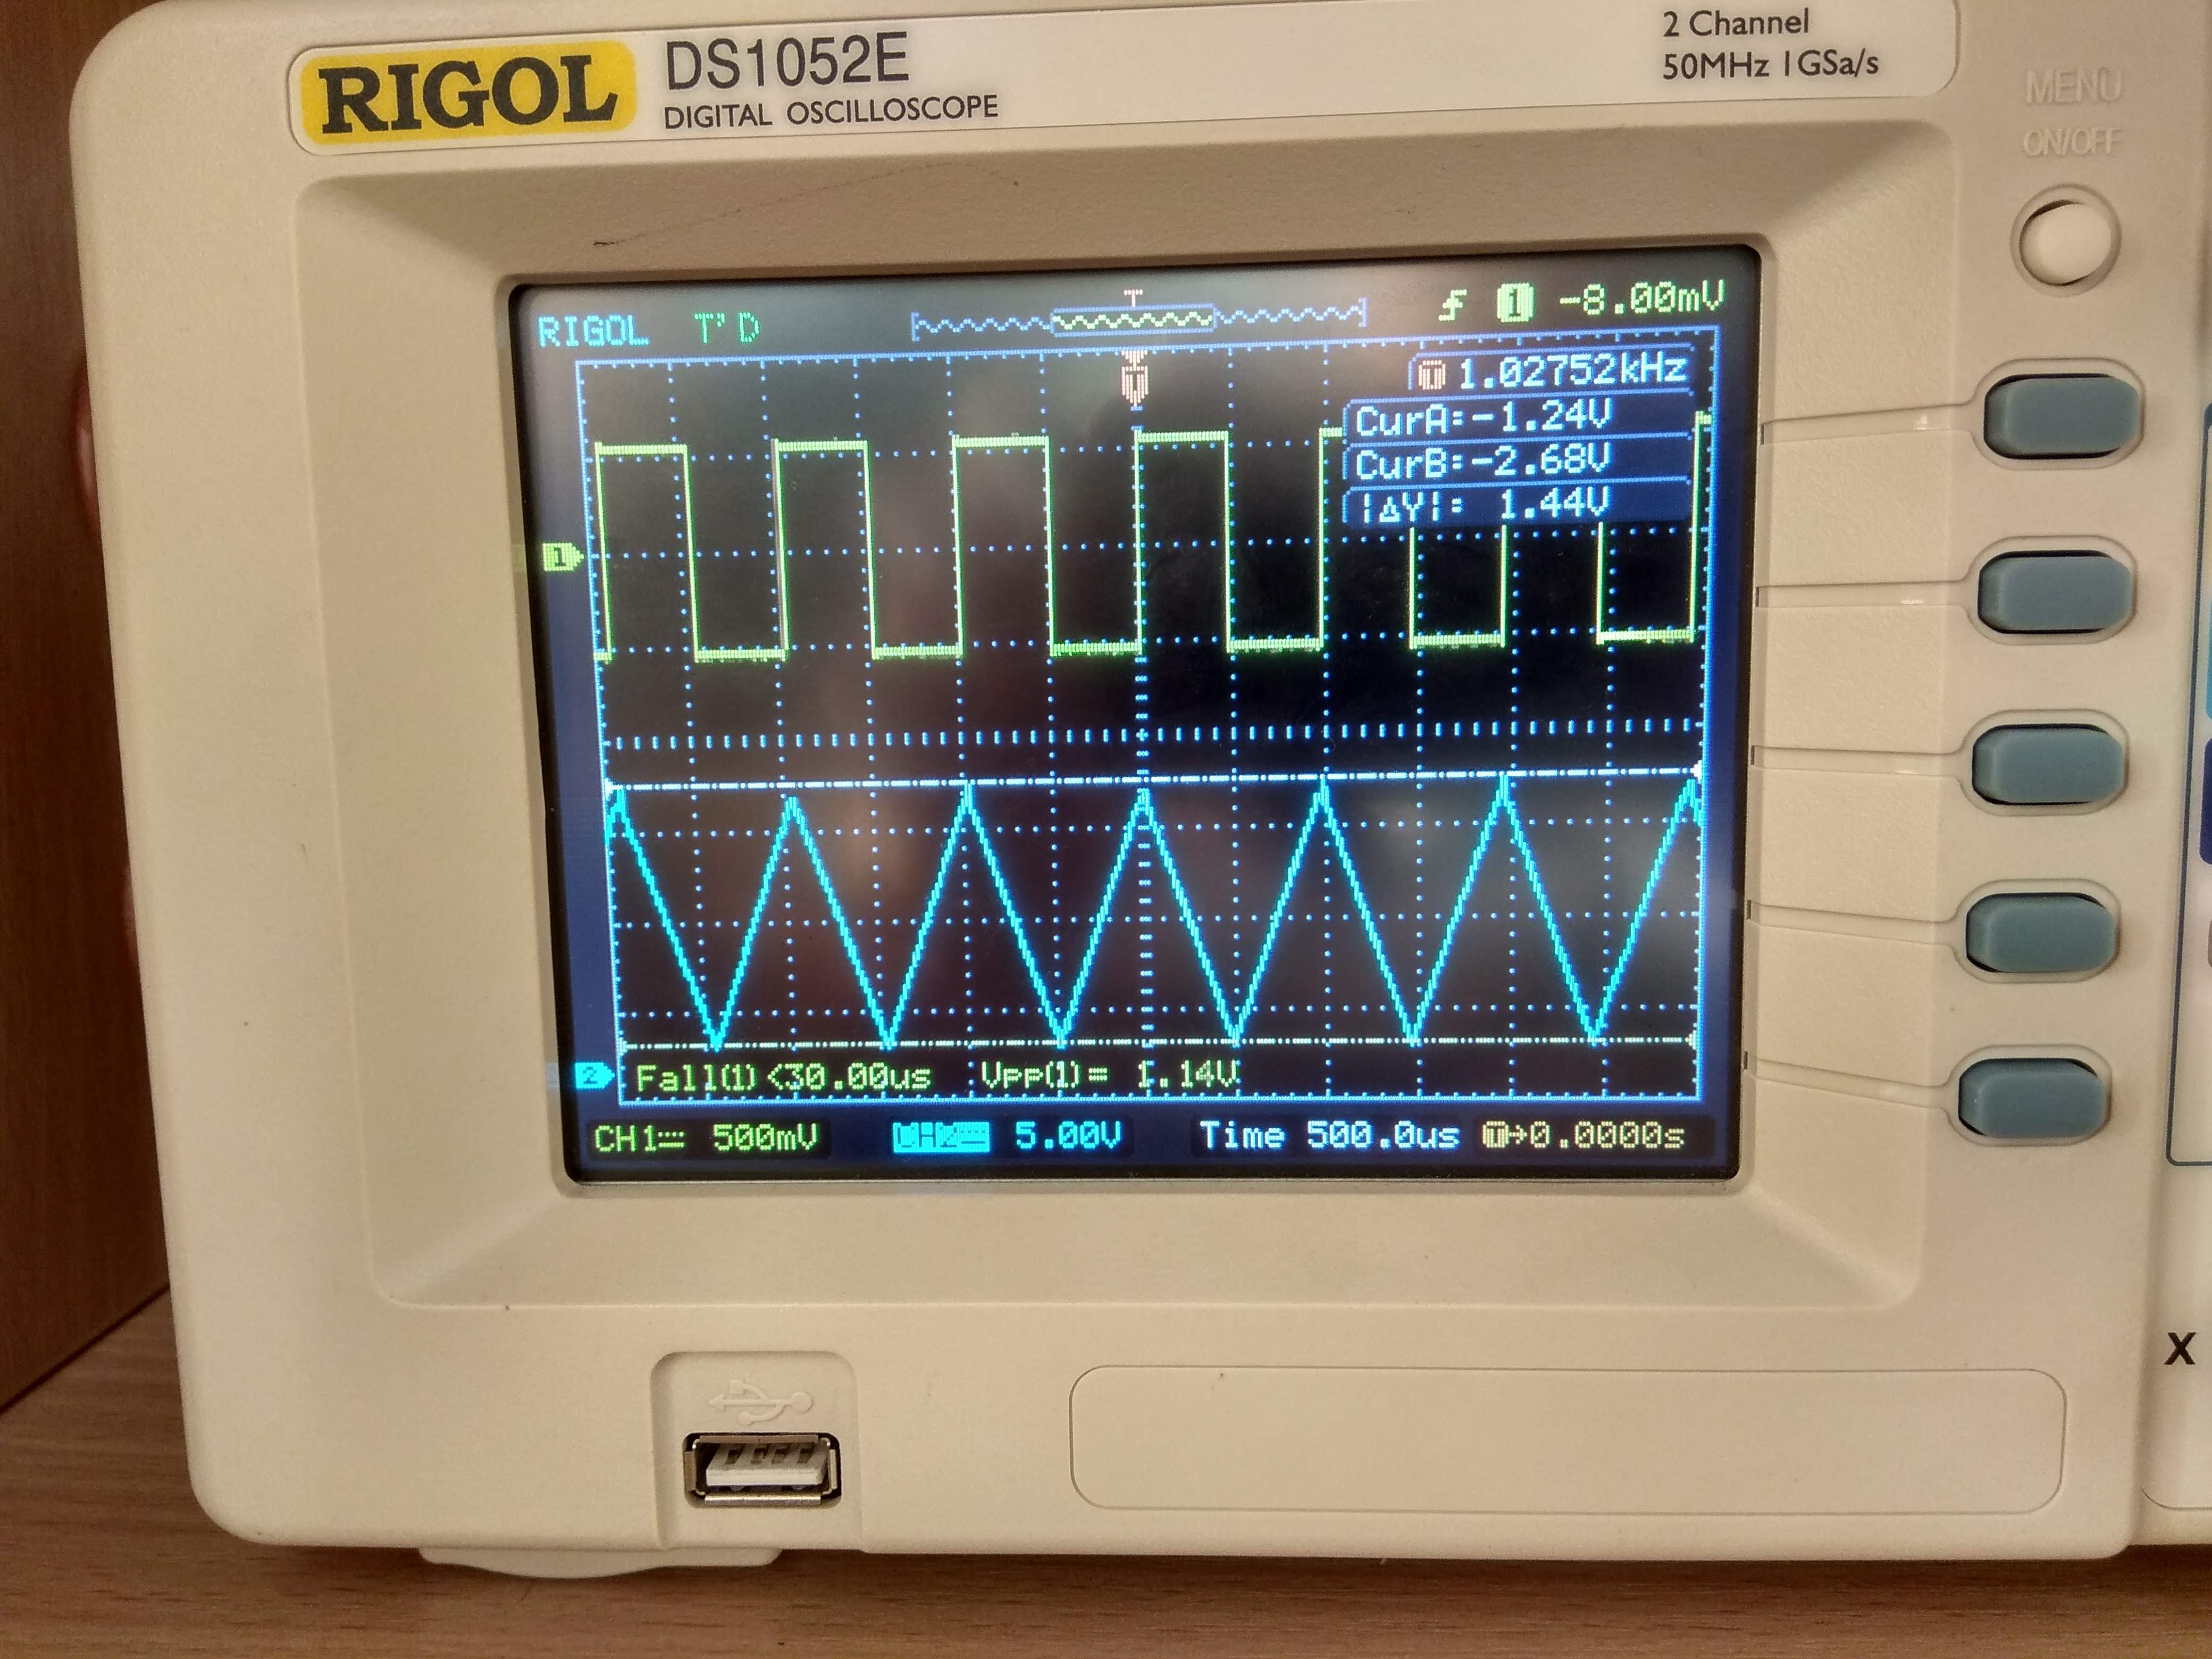
\includegraphics[scale=0.1]{151.jpg}
	\captionof{figure}{Przebieg wejściowy (żółty) i jego całka (niebieski) dla wzmacniacza napięciowego w roli integratora.}
\end{figure}


\subsection{Wnioski}

\section{Blok różniczkujący} %1.4.1

\subsection{Cel zadania}

Badanie układu różniczkującego.

\subsection{Przebieg zadania}

Przygotowano układ zgodnie z instrukcjami i z jego pomocą uzyskano na wyjściu niestabilny przebieg prostokątny ustawiając przełączniki na $3$ dla INPUT i $1,4$ dla LOOPBACK.

\begin{figure}[H]
	\centering
	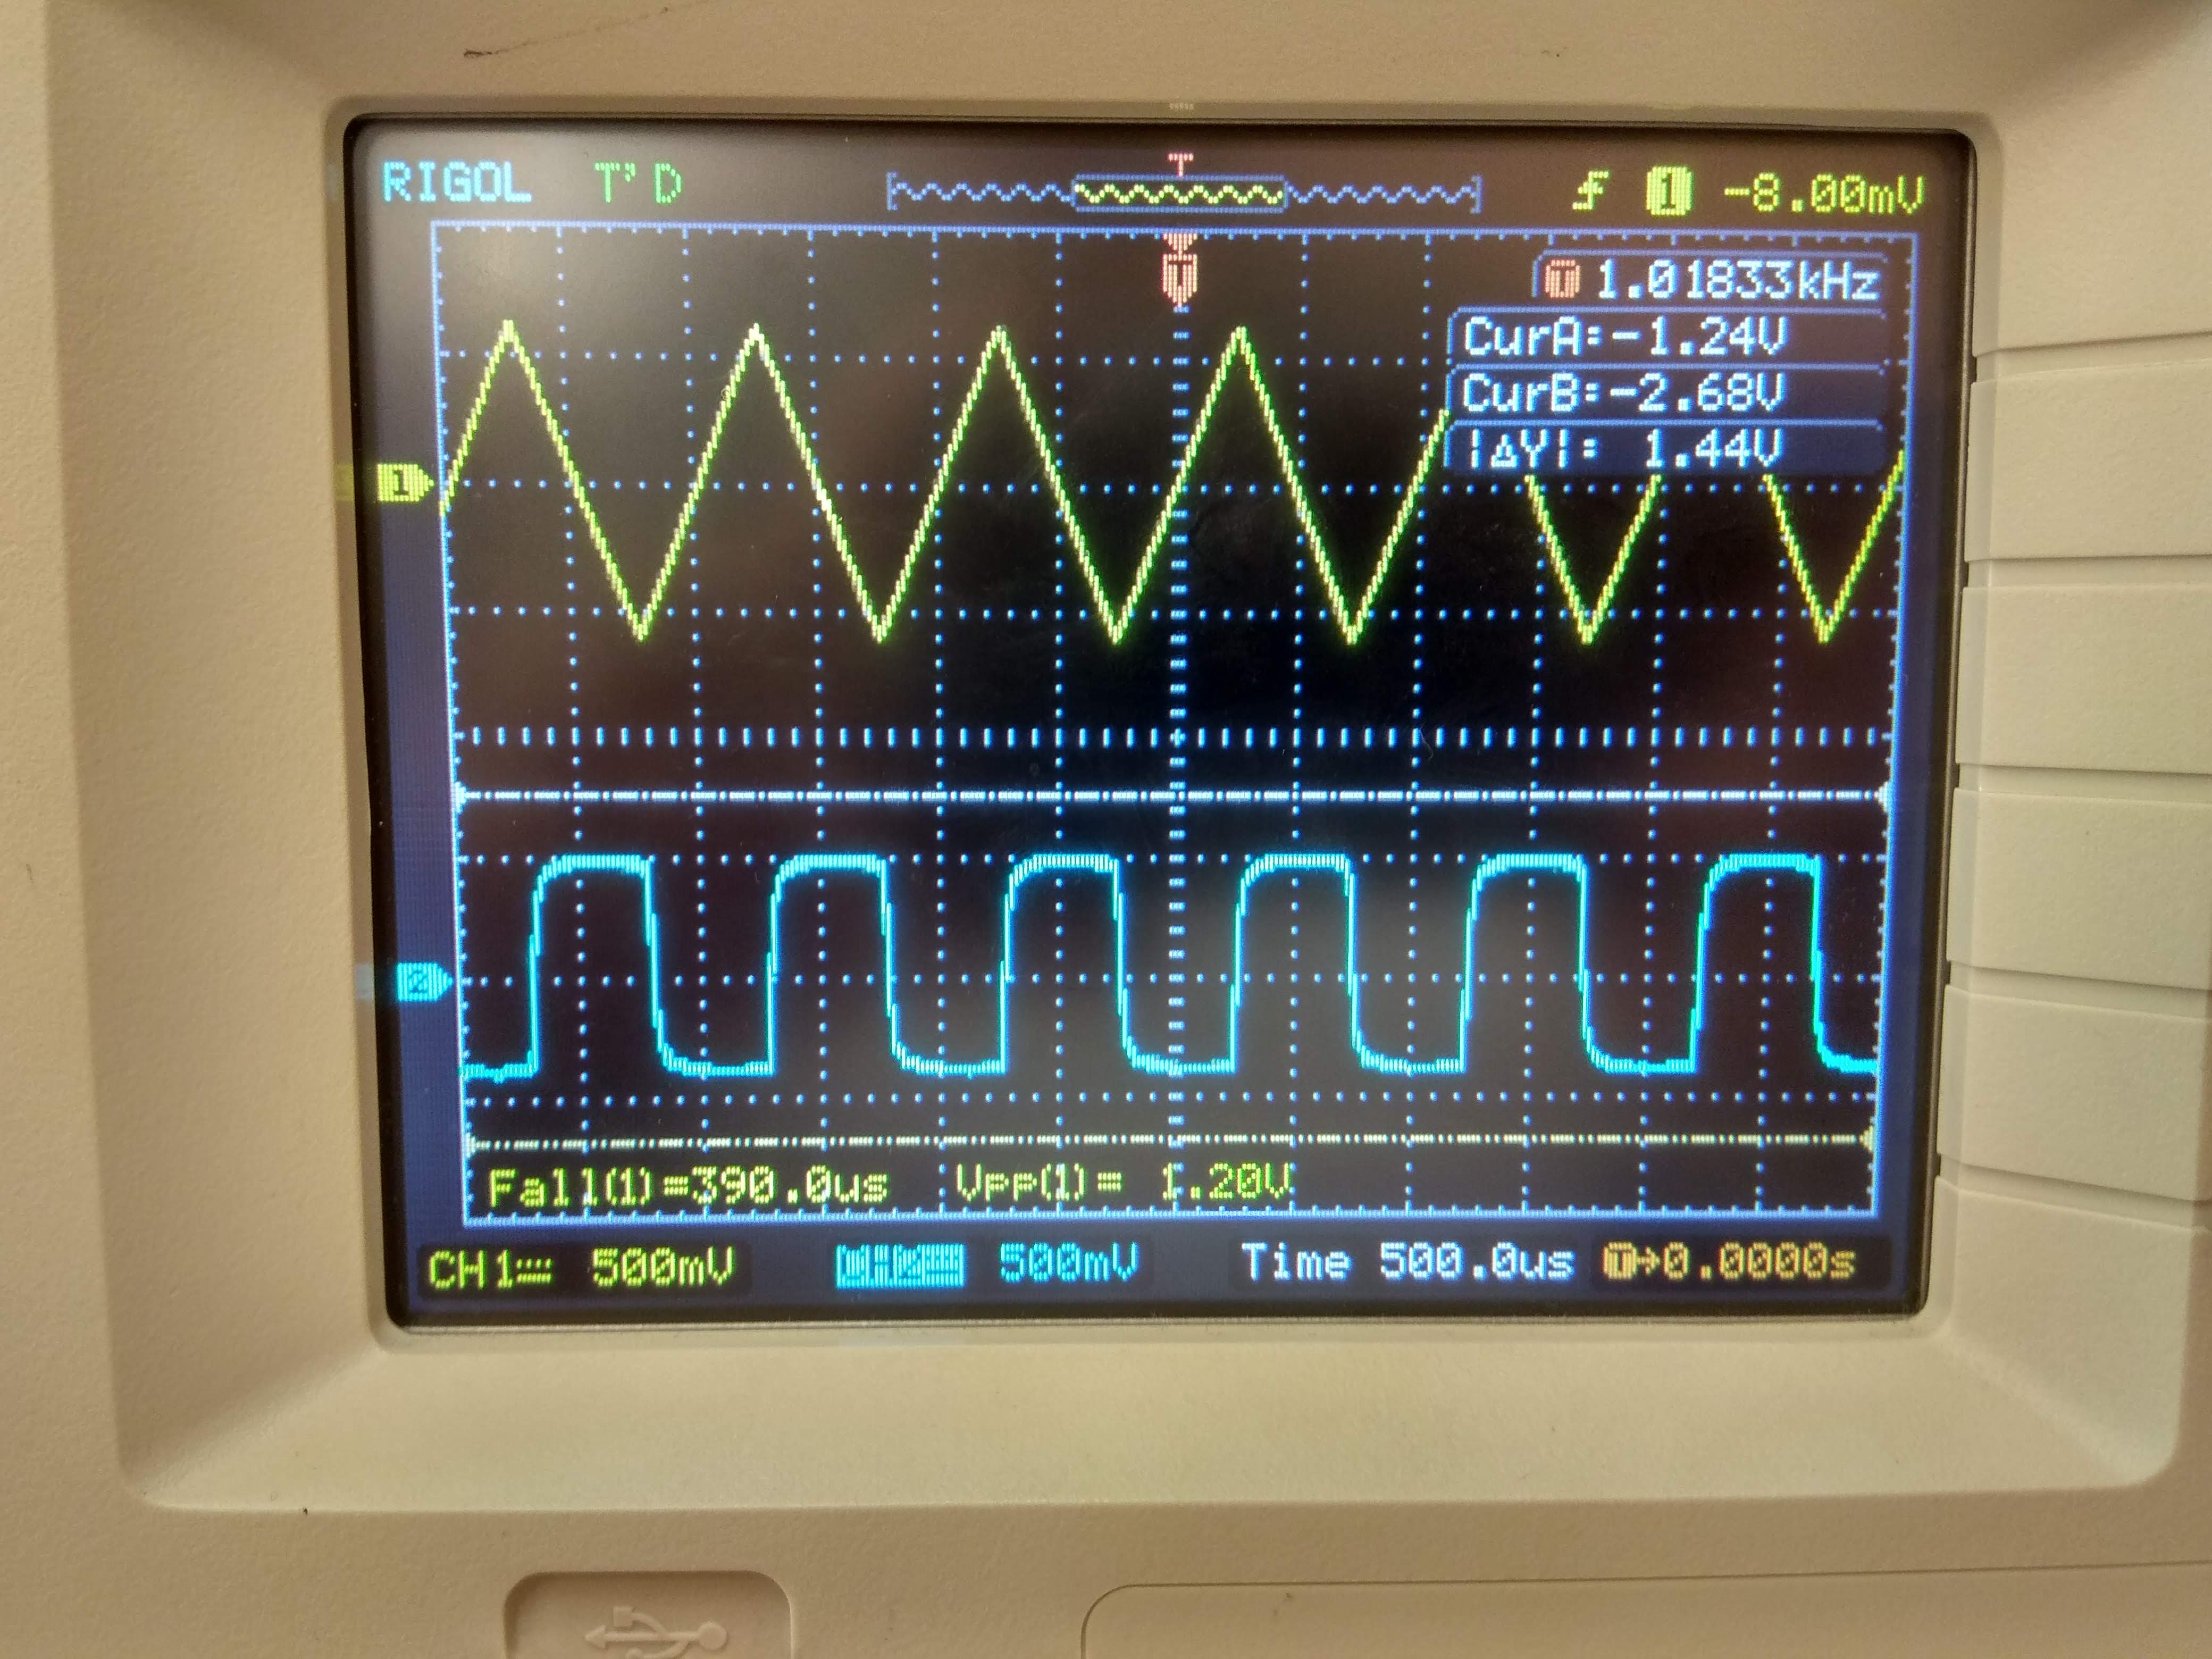
\includegraphics[scale=0.1]{1611.jpg}
	\captionof{figure}{Uzyskany niestabiny przebieg prostokątny (niebieski)}
\end{figure}

Następnie zmieniono ustawienia przełączników na $3$ dla INPUT i $1,4$ dla LOOPBACK, dzięki czemu na  wyjściu otrzymano stabilny przebieg prostokątny.

\begin{figure}[H]
	\centering
	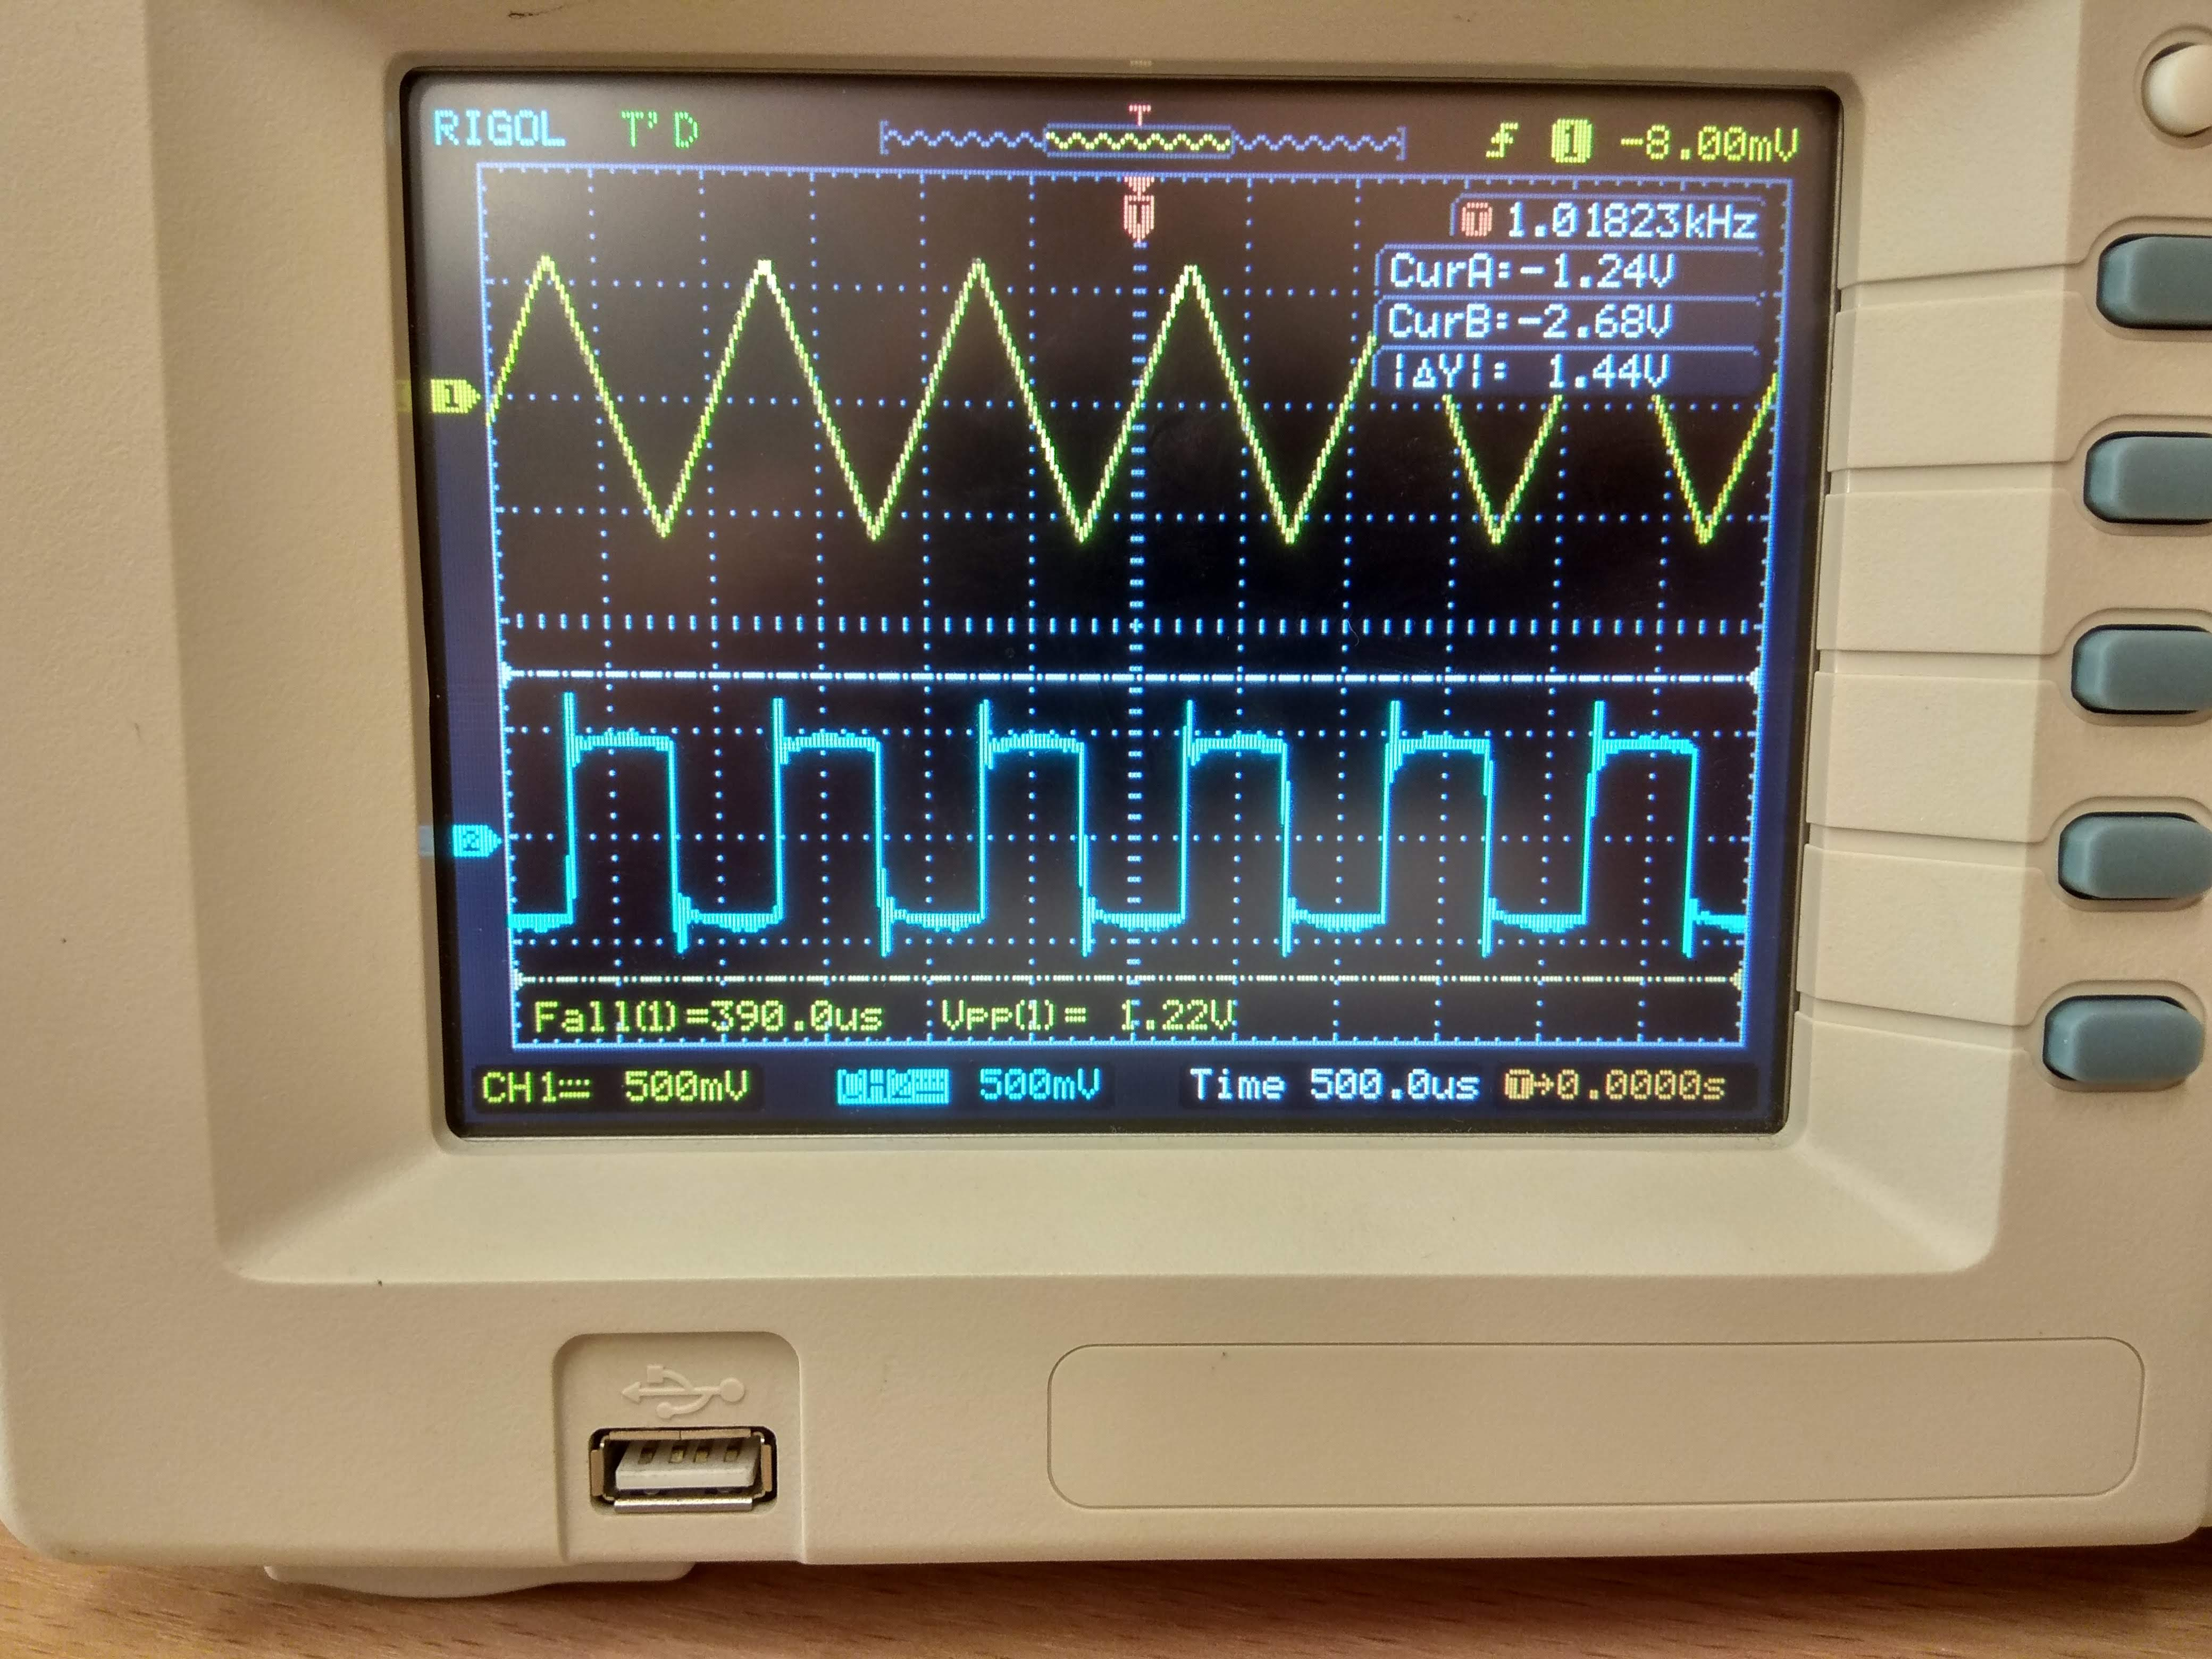
\includegraphics[scale=0.1]{1612.jpg}
	\captionof{figure}{Przebieg wejściowy (żółty) i jego pochodna (niebieski)}
\end{figure}


{\centering
\colorbox{red}{dlaczemu?}}

\subsection{Wnioski}


\end{spacing}

	\begin{thebibliography}{99}


		\bibitem{pa4} Stanisław Bolkowski,  \emph{Elektrotechnika,} WSiP, 2005r.
		
		\bibitem{pa5} Krakowski Maciej,  \emph{Elektrotechnika teoretyczna,} Wydawnictwo Naukowe PWN, 1995r.
		
		\bibitem{pa6} R. Kurdziel,  \emph{Podstawy elektrotechniki,} Wydawnictwo Naukowe WSiP, 1999r.

	\end{thebibliography}
		
	\newpage
	\tableofcontents
		
\end{document}


